% !TEX root = paper/UNI_Sindy.tex

%%%%%%%%%%%%%%%% START OF PREAMBLE %%%%%%%%%%%%%%%

% Basic setup. Authors shouldn't need to adjust these commands.
% It's annoying, but please do NOT strip these into a separate file.
% They need to be included in this .tex for our production software to work.

% Use the basic LaTeX article class, 12pt text
\documentclass[12pt]{article}

% Science uses Times font. If you don't have this installed (most LaTeX installations will be
% fine) or prefer the old Computer Modern fonts, comment out the following line
\usepackage{newtxtext,newtxmath}
% Depending on your LaTeX fonts installation, you might get better results with one or both of these:
%\usepackage{mathptmx}
%\usepackage{txfonts}

% Allow external graphics files
\usepackage{graphicx}

% Use US letter sized paper with 1 inch margins
\usepackage[letterpaper,margin=1in]{geometry}

% Double line spacing, including in captions
\linespread{1.5} % For some reason double spacing is 1.5, not 2.0!

% One space after each sentence
\frenchspacing

% Abstract formatting and spacing - no heading
\renewenvironment{abstract}
	{\quotation}
	{\endquotation}

% No date in the title section
\date{}

% Reference section heading
\renewcommand\refname{References and Notes}

% Figure and Table labels in bold
\makeatletter
\renewcommand{\fnum@figure}{\textbf{Figure \thefigure}}
\renewcommand{\fnum@table}{\textbf{Table \thetable}}
\makeatother

% Call the accompanying scicite.sty package.
% This formats citation numbers in Science style.
\usepackage{scicite}

% Provides the \url command, and fixes a crash if URLs or DOIs contain underscores
\usepackage{url}

%%%%%%%%%%%% CUSTOM COMMANDS AND PACKAGES %%%%%%%%%%%%
% Authors can define simple custom commands e.g. as shortcuts to save on typing
% Use \newcommand (not \def) to avoid overwriting existing commands.
% Keep them as simple as possible and note the warning in the text below.

% Enable color support for TODO markers (remove for final submission)
\usepackage{xcolor}
% Enable strikethrough for version comparison (remove for final submission)
\usepackage{ulem}

\newcommand{\frameworkname}{\textsc{py-xl-sindy}}
\newcommand{\lagrangecat}{\textit{Lagrange}}
\newcommand{\classicalcat}{\textit{Classical}}
\newcommand{\forcescat}{\textit{ExternalForces}}

% TODO command - creates a highly visible TODO marker
\newcommand{\TODO}[1]{\textbf{\textcolor{red}{\Large TODO: \normalsize #1}}}

% Version comparison command - shows old vs new versions with clear visual distinction
\newcommand{\concurrentversion}[2]{%
    \textcolor{red}{#1} \textcolor{blue}{\textbf{#2}}%
}

% Alternative version command that shows both versions in a box for review
\newcommand{\versioncompare}[2]{%
    \fbox{\parbox{\textwidth}{%
        \textcolor{red}{\textbf{OLD:} #1} \\[0.5em]
        \textcolor{blue}{\textbf{NEW:} #2}%
    }}%
}

% AI revised content command - shows AI-revised text in small dark green
\newcommand{\airevised}[1]{\textcolor{olive}{\small #1}}


%%%%%%%%%%%%%%%% TITLE AND AUTHORS %%%%%%%%%%%%%%%%

% Title of the paper.
\def\scititle{
	A Unified Framework for Robust Discovery of Hybrid Physical Dynamics from Data \TODO{change title}
}
% Store the title in a variable for reuse in the supplement (otherwise \maketitle deletes it)
\title{\bfseries \boldmath \scititle}

% Author and institution list.
\author{
	Eymeric Chauchat,$^{1\ast}$
	A.~Collaborator,$^{1,2}$
	Lead Scientist$^{1}$\and
	% Institution list, in a slightly smaller font
	\small$^{1}$Department of Robotics, Graduate School of Engineering, Tohoku University, Sendai, Japan.\and
	\small$^{2}$Another Department, Different Institution, City \& Postal Code, Country.\and
	% Identify at least one corresponding author, with contact email address
	\small$^\ast$Corresponding author. Email: [Your Email Here]\and
	\small$^\dagger$These authors contributed equally to this work.
	\TODO{correctly format, add correct people}
}

%%%%%%%%%%%%%%%%% END OF PREAMBLE %%%%%%%%%%%%%%%%


%%%%%%%%%%%%%%%% START OF MAIN TEXT %%%%%%%%%%%%%%%
\begin{document} 

% Insert the title and author list
\maketitle

% Abstract, in bold
\begin{abstract} \bfseries \boldmath
% The user's original abstract is commented out below, replaced by the AI-revised version as it seems to be the intended one.
% System characterisation is fundamental for understanding the behavior of complex mechanical systems and for their control. New algorithm-based method to discover the dynamics of a system are a revolution from the manual analytical analysis. In this field Sparse Identification of Nonlinear Dynamics is one of the most mature methods. We present here \frameworkname, a unified framework that can perform SINDy system discovery on systems composed of hybrid formalism: Newtonian, Lagrangian and any other heuristic. In the mean time it is also suited for mixed implicit and explicit situation, in the case of not every coordinate activated. We demonstrate the framework's superior performance and robustness on a series of increasing challenging simulated system on MuJoCo.This work provides a powerful, extensible tool for the automated discovery of complex, hybrid physical laws from experimental data.

\airevised{Automated discovery of governing equations for complex mechanical systems is often hindered by methods that cannot handle hybrid physical formalisms or implicit dynamics. To address this, we introduce \frameworkname, a unified computational framework that extends Sparse Identification of Nonlinear Dynamics (SINDy). Our framework's key innovation is a modular catalog that seamlessly combines Lagrangian, Newtonian, and other modeling paradigms to identify hybrid systems from a single data source. It further incorporates a robust, constrained-optimization solver to accurately identify implicit dynamics, even in systems with unforced coordinates. We demonstrate that \frameworkname\ successfully discovers the governing equations for a series of increasingly complex mechanical systems, with models that show high-fidelity agreement with the MuJoCo physics simulator. This work provides a powerful and extensible tool for the automated discovery of complex physical laws from experimental data.}

\TODO{mainly correct need to refine}
\end{abstract}


\noindent
\textbf{TEASER : } A new system identification framework that can handle hybrid physical formalism and implicit/explicit experiments.

% The first paragraph does NOT have a heading, as per Science style.
\noindent
The ability to distill natural laws from observational data into concise mathematical equations is a cornerstone of scientific progress. Recently, data-driven methods, particularly the Sparse Identification of Nonlinear Dynamics (SINDy) framework, have shown great promise in automating this discovery process \cite{Brunton2016_SINDy}. SINDy operates on the assumption of parsimony: that most physical systems are governed by equations with only a few active terms. However, the original SINDy formulation is best suited for explicit, ordinary differential equations in the form $\dot{\mathbf{x}} = f(\mathbf{x})$.

This has led to the development of specialized variants to handle different physical paradigms. For instance, Lagrangian SINDy focuses on identifying the scalar Lagrangian of a system, a more concise representation for many mechanical systems \cite{Chu2020_LagrangianSINDy, Purnomo2023_xLSINDy}. Other variants like SINDy-PI were developed to handle implicit dynamics ($\mathbf{f}(\mathbf{x}, \dot{\mathbf{x}}) = 0$), which are common in constrained mechanical systems or models with rational dynamics, though they can be sensitive to noise \cite{Kaheman2020_SINDyPI}. These methods, while powerful, exist as distinct algorithms, making it difficult to model hybrid systems that might involve, for example, a core Lagrangian structure with additional non-conservative forces best described in a classical framework. In addition, it is likely to find on system an implicit and explict subspace, specificaly concerning robot where not all coordinate are activated. Furthermore, scaling these discovery methods to handle large datasets and enabling their use in modern applications like reinforcement learning requires a focus on computational efficiency.

Here, we introduce \frameworkname, a comprehensive and extensible Python framework that unifies these disparate approaches and addresses their limitations. Our main contributions are:
\begin{itemize}
    \item \textbf{A Unified Hybrid Modeling Framework:} We introduce a modular catalog architecture that allows for the seamless combination of different physical models. Users can construct a single regression problem from `Lagrange`, `Classical` (Newtonian), and `ExternalForces` components, enabling the discovery of hybrid dynamics.
    \item \textbf{Robust Implicit Dynamics Identification:} We implement a robust solver for implicit dynamics based on constrained optimization, inspired by SINDy-PI, and introduce a novel post-processing algorithm to automatically cluster and identify the true sparse solution from the resulting coefficient matrix.
    \item \textbf{High-Performance Parallelization:} The framework is integrated with JAX, enabling JIT-compilation and auto-vectorization (`vmap`) of the dynamics functions. This allows for massive parallelization of simulations, critical for large-scale hyperparameter searches, uncertainty quantification, and integration with machine learning pipelines.\TODO{Not clear and not really true}
    \item \textbf{End-to-End Validation Pipeline:} We present a complete workflow for generating data from the high-fidelity MuJoCo simulator, performing the system identification, and validating the discovered models against the simulator's trajectory, providing a robust metric for real-world performance.
\end{itemize}
\TODO{Overall, clear but need to be refined... }

\section*{Methods}

This work is a combinaison of previously developped algorithm and new addition from \frameworkname. Before diving into the newer method, we will give indepth explanation of the past method. The new unified algorithm has been developped by mixing Sindy and Lagrangian \cite{purnomoSparseIdentificationLagrangian2023} catalog and also mixing the Explicit and Implicit discovery.

\subsection*{SINDy catalog}

\TODO{General SINDY catalog definition}

\subsection*{The Unified Catalog Framework}

The core of \frameworkname\ is its modular catalog system. We implemented three main categories:
\begin{itemize}
    \item \textbf{\lagrangecat:} This category takes a library of candidate symbolic functions and constructs the experimental matrix by applying the Euler-Lagrange operator, $\frac{d}{dt}\frac{\partial L}{\partial \dot{q}_i} - \frac{\partial L}{\partial q_i}$.
    \item \textbf{\classicalcat:} This category represents standard Newtonian or state-space models. It takes a library of functions of the state variables (e.g., polynomials, trigonometric functions) and constructs the corresponding columns in the experimental matrix directly.
    \item \textbf{\forcescat:} This category explicitly models external forces, typically serving as the known right-hand-side of the final governing equation.
\end{itemize}
The `CatalogRepartition` class combines instances of these categories into a single, cohesive experimental matrix $\mathbf{\Theta}$. This allows for the construction of a hybrid equation, for example $\mathbf{M}(\mathbf{q})\ddot{\mathbf{q}} + \mathbf{C}(\mathbf{q},\dot{\mathbf{q}})\dot{\mathbf{q}} + \mathbf{g}(\mathbf{q}) = \mathbf{\tau} + \mathbf{F}_{friction}(\dot{\mathbf{q}})$, where the Lagrangian terms are handled by the `Lagrange` catalog and the friction terms by the `Classical` catalog.

\subsection*{Explicit regression}

\TODO{Talk about LassoCV and explicit regression}

\subsection*{Implicit regression}

\TODO{Talk about Implicit regression and CVxPY}

\subsection*{mixed regression}

\TODO{Talk about the agregation of explicit and implicit regression method}


\section*{Results}

\subsection*{Catalog generation}

In order to compare regression that uses different base catalog it is important to generate equivalent catalog following a criteria. For the xlsindy catalog we have generated all the combination of the following polynome : 
\TODO{list polynome}

Concerning the sindy catalog, we have decided to help it as much as possible and we have decided to choose the minimum polynome generate that lead to a catalog that include all the polynome formed by euler lagrange equation in the xlsindy case (we have the catalog of the mininum size that include the catalog resulted by the euler lagrange transform of the xlsindy catalog)\TODO{not really clear right now.......}

\subsection*{Experiment Results}

In order to validate the capabilities of \frameworkname, we conducted a series of experiments on mechanical systems of increasing complexity. All data were generated using the MuJoCo physics simulator, with random time-varying external forces applied to ensure rich exploration of the state space. The generated datasets were then used to identify the governing equations using our framework, and the discovered models were validated by comparing their simulated trajectories against those from MuJoCo.

We have focused on three main systems:
\begin{enumerate}
	\item Cart-pole
	\item Double pendulum ( point mass )
	\item Double pendulum (point mass ) on a cart
\end{enumerate}

On these three systems, we have generated multiple trajectory with different friction coefficient, and different input forces profile. We have divided the input forces into implicit (no forces on the system, only initial condition), explicit (forces on every actuated joint) and mixed (forces on a subset of the joint). 
On this dataset we have added multiple level of gaussian noise to the position, velocity and acceleration. Finally we have run the different configuration of \frameworkname\ to identify the system. The same level of resources has been allocated to each configuration and a timeout of 1h has been set for each run.
The list of framework is the following: 
\begin{enumerate}
	\item mixed catalog (Lagrange + classical) X mixed implicit/explicit solver
	\item mixed catalog (Lagrange + classical) X explicit solver
	\item mixed catalog (Lagrange + classical) X implicit solver
	\item Lagrange catalog X mixed implicit/explicit solver
	\item Lagrange catalog X explicit solver
	\item Lagrange catalog X implicit solver
	\item classical catalog X mixed implicit/explicit solver
	\item classical catalog X explicit solver
	\item classical catalog X implicit solver 
\end{enumerate}

After obtaining the different models, we have generated a validation trajectory with Mujoco and compared the trajectory of the discorvered model with the one of Mujoco. Using this metric we have ranked the different configuration of \frameworkname. 

For each of the trajectory (with a fixed noise level) the different framework configuration are compared with each other, and ranked from best to worst. A special award is given if a configuration is the only one to find a valid model (able to create a validation trajectory that doesn't diverge) called "Wins without competition" (Wins WC). The results are summarized in Table \ref{tab:results_summary} and ranked by number of 1st place wins.

\begin{table}[h]
\centering
\caption{Overall Performance Ranking (by number of 1st place wins)}
\label{tab:results_summary}
\small
\begin{tabular}{clccccccccc}
\hline
\textbf{Rank} & \textbf{Combo} & \textbf{Win Rate} & \textbf{Wins WC} & \textbf{Total} & \textbf{1st} & \textbf{2nd} & \textbf{3rd} & \textbf{$>$ 3rd} & \textbf{Timeout} & \textbf{Other Fail} \\
\hline
1 & mixed $\times$ mixed (our)& 0.595 & 26 & 116 & 69.0 & 22.0 & --- & 0 & 0 & 25 \\
2 & mixed $\times$ explicit& 0.674 & 23 & 92 & 62.0 & 16.0 & --- & 0 & 0 & 14 \\
3 & sindy $\times$ explicit & 0.239 & 1 & 92 & 22.0 & 8.0 & 1.0 & 0 & 16 & 45 \\
4 & sindy $\times$ mixed & 0.170 & 1 & 112 & 19.0 & 11.0 & 1.0 & 0 & 43 & 38 \\
5 & mixed $\times$ implicit & 0.625 & 4 & 16 & 10.0 & 3.0 & 2.0 & 0 & 0 & 1 \\
6 & xlsindy $\times$ explicit & 0.054 & 3 & 92 & 5.0 & 35.0 & 12.0 & 2 & 0 & 38 \\
7 & xlsindy $\times$ mixed & 0.043 & 3 & 115 & 5.0 & 37.0 & 14.0 & 0 & 0 & 59 \\
8 & xlsindy $\times$ implicit & 0.600 & 1 & 5 & 3.0 & 1.0 & 1.0 & 0 & 0 & 0 \\
9 & sindy $\times$ implicit & 0.000 & 0 & 24 & --- & --- & --- & 0 & 23 & 1 \\
\hline
\end{tabular}
\end{table}

Our developped method (mixed catalog X mixed implicit/explicit solver) is the best performing one, winning 69 out of 116 trajectory (59.5\% win rate) and being the only one to find a valid model on 26 trajectory. The second best method (mixed catalog X explicit solver) is also using the mixed catalog but only the explicit solver. The third best method (classical catalog X explicit solver) is using only the classical catalog, as it can been seen the greater size of catalog usually leads to more timeouts. 
The main reason of why xlsindy is not performing well is because it is not able to handle well the friction term and majority of the experiment have friction.


\section*{Discussion}
In this work, we presented \frameworkname, a novel framework that unifies and extends the capabilities of Sparse Identification of Nonlinear Dynamics. By introducing a modular, hybrid catalog system, we have bridged the gap between Lagrangian and Newtonian formulations, allowing for the discovery of more realistic physical models that include both conservative and dissipative forces. Our implementation of a robust implicit solver with automated post-processing expands the class of systems that can be identified to include those with complex constraints.

The integration with JAX for high-performance computing is a key practical advance, making it feasible to apply these discovery techniques to large-scale problems. Our end-to-end pipeline, which uses the MuJoCo simulator for data generation and validation, ensures that the discovered models are not just theoretically sound but are benchmarked against a realistic physics engine.

Limitations of our current framework include the need for the user to design the initial candidate library of functions, a common challenge in all SINDy-based methods. Future work will focus on automating this library construction process and integrating the high-performance dynamics models into model-based reinforcement learning algorithms, paving the way for agents that can not only learn to control a system but also discover its underlying physical laws.
\TODO{don't talk about jax, it is too implementation related...}

\newpage

%%%%%%%%%%%%%%%% MAIN TEXT FIGURES %%%%%%%%%%%%%%%

\begin{figure}
	\centering
	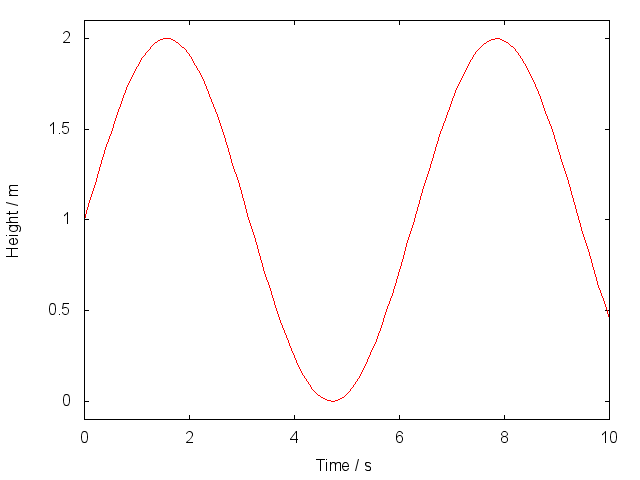
\includegraphics[width=0.9\textwidth]{placeholder.png}
	\caption{\textbf{Validation of a discovered hybrid model for a cart-pole with friction.} 
    (\textbf{A}) Comparison of trajectories for the generalized coordinates (position and angle) between the ground-truth MuJoCo simulation (black dashed line) and the model discovered by \frameworkname\ (blue solid line). (\textbf{B}) Residuals between the MuJoCo and discovered model trajectories, showing high fidelity. (\textbf{C}) The discovered coefficient vector, showing sparse non-zero terms corresponding to the correct Lagrangian and friction functions.}
	\label{fig:trajectory_validation}
\end{figure}

\begin{figure}
	\centering
	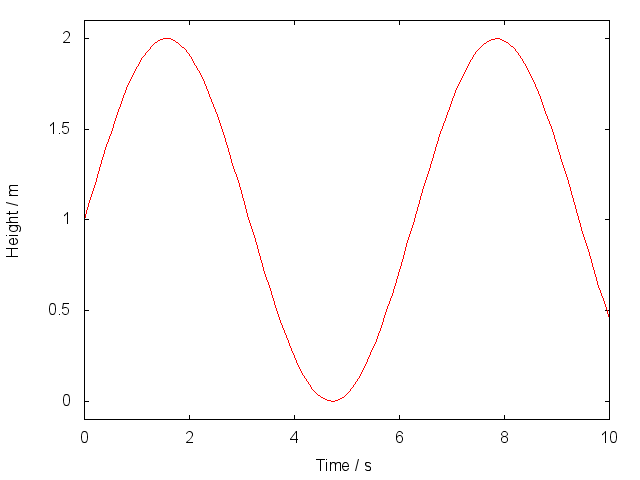
\includegraphics[width=0.9\textwidth]{placeholder.png}
	\caption{\textbf{Implicit identification of a double pendulum on a cart.} 
    (\textbf{A}) The solution matrix `X` from the constrained optimization problem. Most columns are sparse. (\textbf{B}) Post-processing identifies a cluster of homothetic column vectors (highlighted in red) that correspond to the true physical law. (\textbf{C}) The final, single solution vector extracted from the cluster, accurately representing the system's implicit dynamics.}
	\label{fig:implicit_results}
\end{figure}


%%%%%%%%%%%%%%%% MAIN TEXT TABLES %%%%%%%%%%%%%%%

\begin{table}
	\centering
	\caption{\textbf{Performance benchmark of JAX-based parallelized dynamics function.}
    Comparison of average computation time per simulation step for a double pendulum model. The JAX implementation is benchmarked on both CPU and GPU, showing orders-of-magnitude speedup when simulating large batches in parallel.}
	\label{tab:jax_performance}
	
	\begin{tabular}{lccc}
		\\
		\hline
		Implementation & Batch Size & Hardware & Avg. Time per Step (ms) \\
		\hline
		NumPy (sequential) & 1 & CPU & $\sim$0.15 \\
		JAX (sequential) & 1 & CPU & $\sim$0.16 \\
		JAX (parallelized) & 10,000 & GPU & $\sim$0.0002 \\
		\hline
	\end{tabular}
\end{table}


%%%%%%%%%%%%%%%% REFERENCES %%%%%%%%%%%%%%%

\clearpage % Clear all remaining figures and tables then start a new page

% Bibliography - replace with your .bib file
\bibliography{UNI_Sindy.bib} % for a file named science_template.bib
\bibliographystyle{sciencemag}


%%%%%%%%%%%%%%%% ACKNOWLEDGEMENTS %%%%%%%%%%%%%%%

\section*{Acknowledgments}
\paragraph*{Funding:}
[TODO: List your funding sources here. Example: This work was supported by the JSPS Grant-in-Aid for Scientific Research (B) under Grant 18H01399.]
\paragraph*{Author contributions:}
E.C. conceived the idea, developed the software, performed the experiments, and wrote the manuscript. A.C. assisted with... L.S. supervised the project... [TODO: Fill out contributions.]
\paragraph*{Competing interests:}
The authors declare no competing interests.
\paragraph*{Data and materials availability:}
All code for the \frameworkname\ framework and the scripts to reproduce the experiments are publicly available on GitHub at \url{https://github.com/Eymeric65/py-xl-sindy}. All data used in this study was generated using the provided code and the MuJoCo simulator. \TODO{ add information about the .sh script used for generating the material.}


%%%%%%%%%%%%%%%% SUPPLEMENT LIST %%%%%%%%%%%%%%%

% List the contents of your Supplementary Materials
\subsection*{Supplementary materials}
Materials and Methods\\
Supplementary Text\\
Figs. S1 to S2\\
Tables S1 to S2\\

%%%%%%%%%%%%%%%% END OF MAIN TEXT %%%%%%%%%%%%%%%

\newpage

%%%%%%%%%%%%%%%% START OF SUPPLEMENT %%%%%%%%%%%%%%%

% Figures, tables, equations and pages in the supplement are numbered S1, S2 etc.
\renewcommand{\thefigure}{S\arabic{figure}}
\renewcommand{\thetable}{S\arabic{table}}
\renewcommand{\theequation}{S\arabic{equation}}
\renewcommand{\thepage}{S\arabic{page}}
\setcounter{figure}{0}
\setcounter{table}{0}
\setcounter{equation}{0}
\setcounter{page}{1} % not 0 as \newpage already started a supplementary page
% References continue the numbering from the main text.


%%%%%%%%%%%%%%%% SUPPLEMENT TITLE PAGE %%%%%%%%%%%%%%%

\begin{center}
\section*{Supplementary Materials for\\ \scititle}

% Author list for the supplement
Eymeric Chauchat,$^{\ast}$ A.~Collaborator, Lead Scientist\\
\small$^\ast$Corresponding author. Email: [Your Email Here]
\end{center}

\subsection*{This PDF file includes:}
Materials and Methods\\
Supplementary Text\\
Figures S1 to S2\\
Tables S1 to S2

\newpage

%%%%%%%%%%%%%%%% MATERIALS AND METHODS %%%%%%%%%%%%%%%

\section*{Materials and Methods}

\subsection*{The Unified Catalog Framework}
The core of \frameworkname\ is its modular catalog system, defined in `src/xlsindy/catalog.py`. The abstract base class `CatalogCategory` defines a standard interface for different physical paradigms. We implemented three main categories:
\begin{itemize}
    \item \textbf{\lagrangecat:} This category takes a library of candidate symbolic functions and constructs the experimental matrix by applying the Euler-Lagrange operator, $\frac{d}{dt}\frac{\partial L}{\partial \dot{q}_i} - \frac{\partial L}{\partial q_i}$.
    \item \textbf{\classicalcat:} This category represents standard Newtonian or state-space models. It takes a library of functions of the state variables (e.g., polynomials, trigonometric functions) and constructs the corresponding columns in the experimental matrix directly.
    \item \textbf{\forcescat:} This category explicitly models external forces, typically serving as the known right-hand-side of the final governing equation.
\end{itemize}
The `CatalogRepartition` class combines instances of these categories into a single, cohesive experimental matrix $\mathbf{\Theta}$. This allows for the construction of a hybrid equation, for example $\mathbf{M}(\mathbf{q})\ddot{\mathbf{q}} + \mathbf{C}(\mathbf{q},\dot{\mathbf{q}})\dot{\mathbf{q}} + \mathbf{g}(\mathbf{q}) = \mathbf{\tau} + \mathbf{F}_{friction}(\dot{\mathbf{q}})$, where the Lagrangian terms are handled by the `Lagrange` catalog and the friction terms by the `Classical` catalog.

\subsection*{Sparse Regression Techniques}
The framework solves the sparse regression problem $\mathbf{b} = \mathbf{\Theta}\mathbf{\Xi}$ to find the coefficient vector $\mathbf{\Xi}$. Two primary solvers are implemented in `src/xlsindy/optimization.py`:
\begin{itemize}
    \item \textbf{Hard Thresholding (STLSQ):} An iterative method where a standard least-squares solution is computed, and then coefficients below a certain threshold are pruned. The process is repeated on the reduced library until the solution converges.
    \item \textbf{Lasso Regression:} Utilizes the L1 regularizer to promote sparsity, implemented via Scikit-learn's `LassoCV` to automatically select the optimal regularization parameter $\alpha$.
\end{itemize}

\subsection*{Implicit Dynamics Identification}
For implicit systems, where no term can be isolated on the left-hand side, we seek a sparse vector $\mathbf{\Xi}$ in the null space of $\mathbf{\Theta}(\mathbf{q}, \dot{\mathbf{q}}, \ddot{\mathbf{q}})=0$. Following the robust approach of SINDy-PI \cite{Kaheman2020_SINDyPI}, we solve a constrained optimization problem using `cvxpy`. The problem is formulated as:
\begin{equation}
	\min_{\mathbf{X}} ||\mathbf{\Theta X} - \mathbf{\Theta}||_F + \lambda||\mathbf{X}||_1 \quad \text{s.t.} \quad \text{diag}(\mathbf{X}) = 0.
\end{equation}

The resulting solution matrix $\mathbf{X}$ ideally contains multiple column vectors that are sparse and homothetic (i.e., pointing in the same direction), representing the same physical law. Our post-processing algorithm in `\_implicit\_post\_treatment` clusters these vectors based on angular similarity and extracts the principal direction via SVD to yield a single, robust solution vector.

\subsection*{Data Generation from MuJoCo Simulator}
All training and validation data were generated using the MuJoCo physics simulator. The scripts in the `util/` directory manage this process.
\begin{enumerate}
    \item \textbf{Data Generation (`mujoco\_generate\_data.py`):} A simulation is run for a specified duration (`max\_time`). At each step, a randomly generated, time-varying external force is applied to the system's actuators. The force is generated using a sum of sinusoids with varying frequencies and amplitudes to ensure sufficient exploration of the state space.
    \item \textbf{Coordinate Transformation (`xlsindy\_gen.py` files):} MuJoCo often uses a different set of generalized coordinates than the standard textbook Lagrangian formulation (e.g., cumulative angles). Each experiment folder contains a `mujoco\_transform` function to convert the simulator's output (`qpos`, `qvel`, `qacc`) into the coordinate system used for the symbolic model.
    \item \textbf{Data Storage:} The generated time-series data is saved to `.npz` files, while simulation metadata is saved to corresponding `.json` files. A validation database (`validation\_database.pkl`) is created by subsampling from all generated experiments to test the generalization of discovered models.
\end{enumerate}

\end{document}
% End of the merged tex file